

\documentclass[../../e1_tp1_main.tex]{subfiles}

\begin{document}
\chapter{Curvas características}
Se busca simular las curvas características de distintos dispositivos y corroborar estas simulaciones con las mediciones obtenidas:

\begin{enumerate}
	\item Diodo común
	\item Diodo Zener
	\item Transistor bipolar
\end{enumerate}

Todas las simulaciones fueron realizadas en LTSPICE. 

\section{Curva del diodo común}
	El diodo utilizado fue el 1N4007, para el cual la tensión de breakdown es de -1000V y su tensión threshold es cercana a los 0.7 V\par
		Se utilizó una fuente de tensión continua, a la cual se la fue variando y se midió la tensión en el diodo y la corriente que circulaba por la resistencia con tester.\par
	El circuito propuesto para realizar las mediciones es el siguiente:
	
	\begin{figure}[H]	%diodo, circuito propuesto
		\centering
		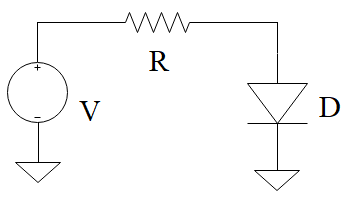
\includegraphics[scale=1.2]{imagenes/circuito_diode.png}
		\caption{Circuito propuesto para las mediciones del diodo.}
		\label{fig:ej5_circuito_diode}
	\end{figure}


\begin{figure}[H]	%diodo, curva
	\centering
	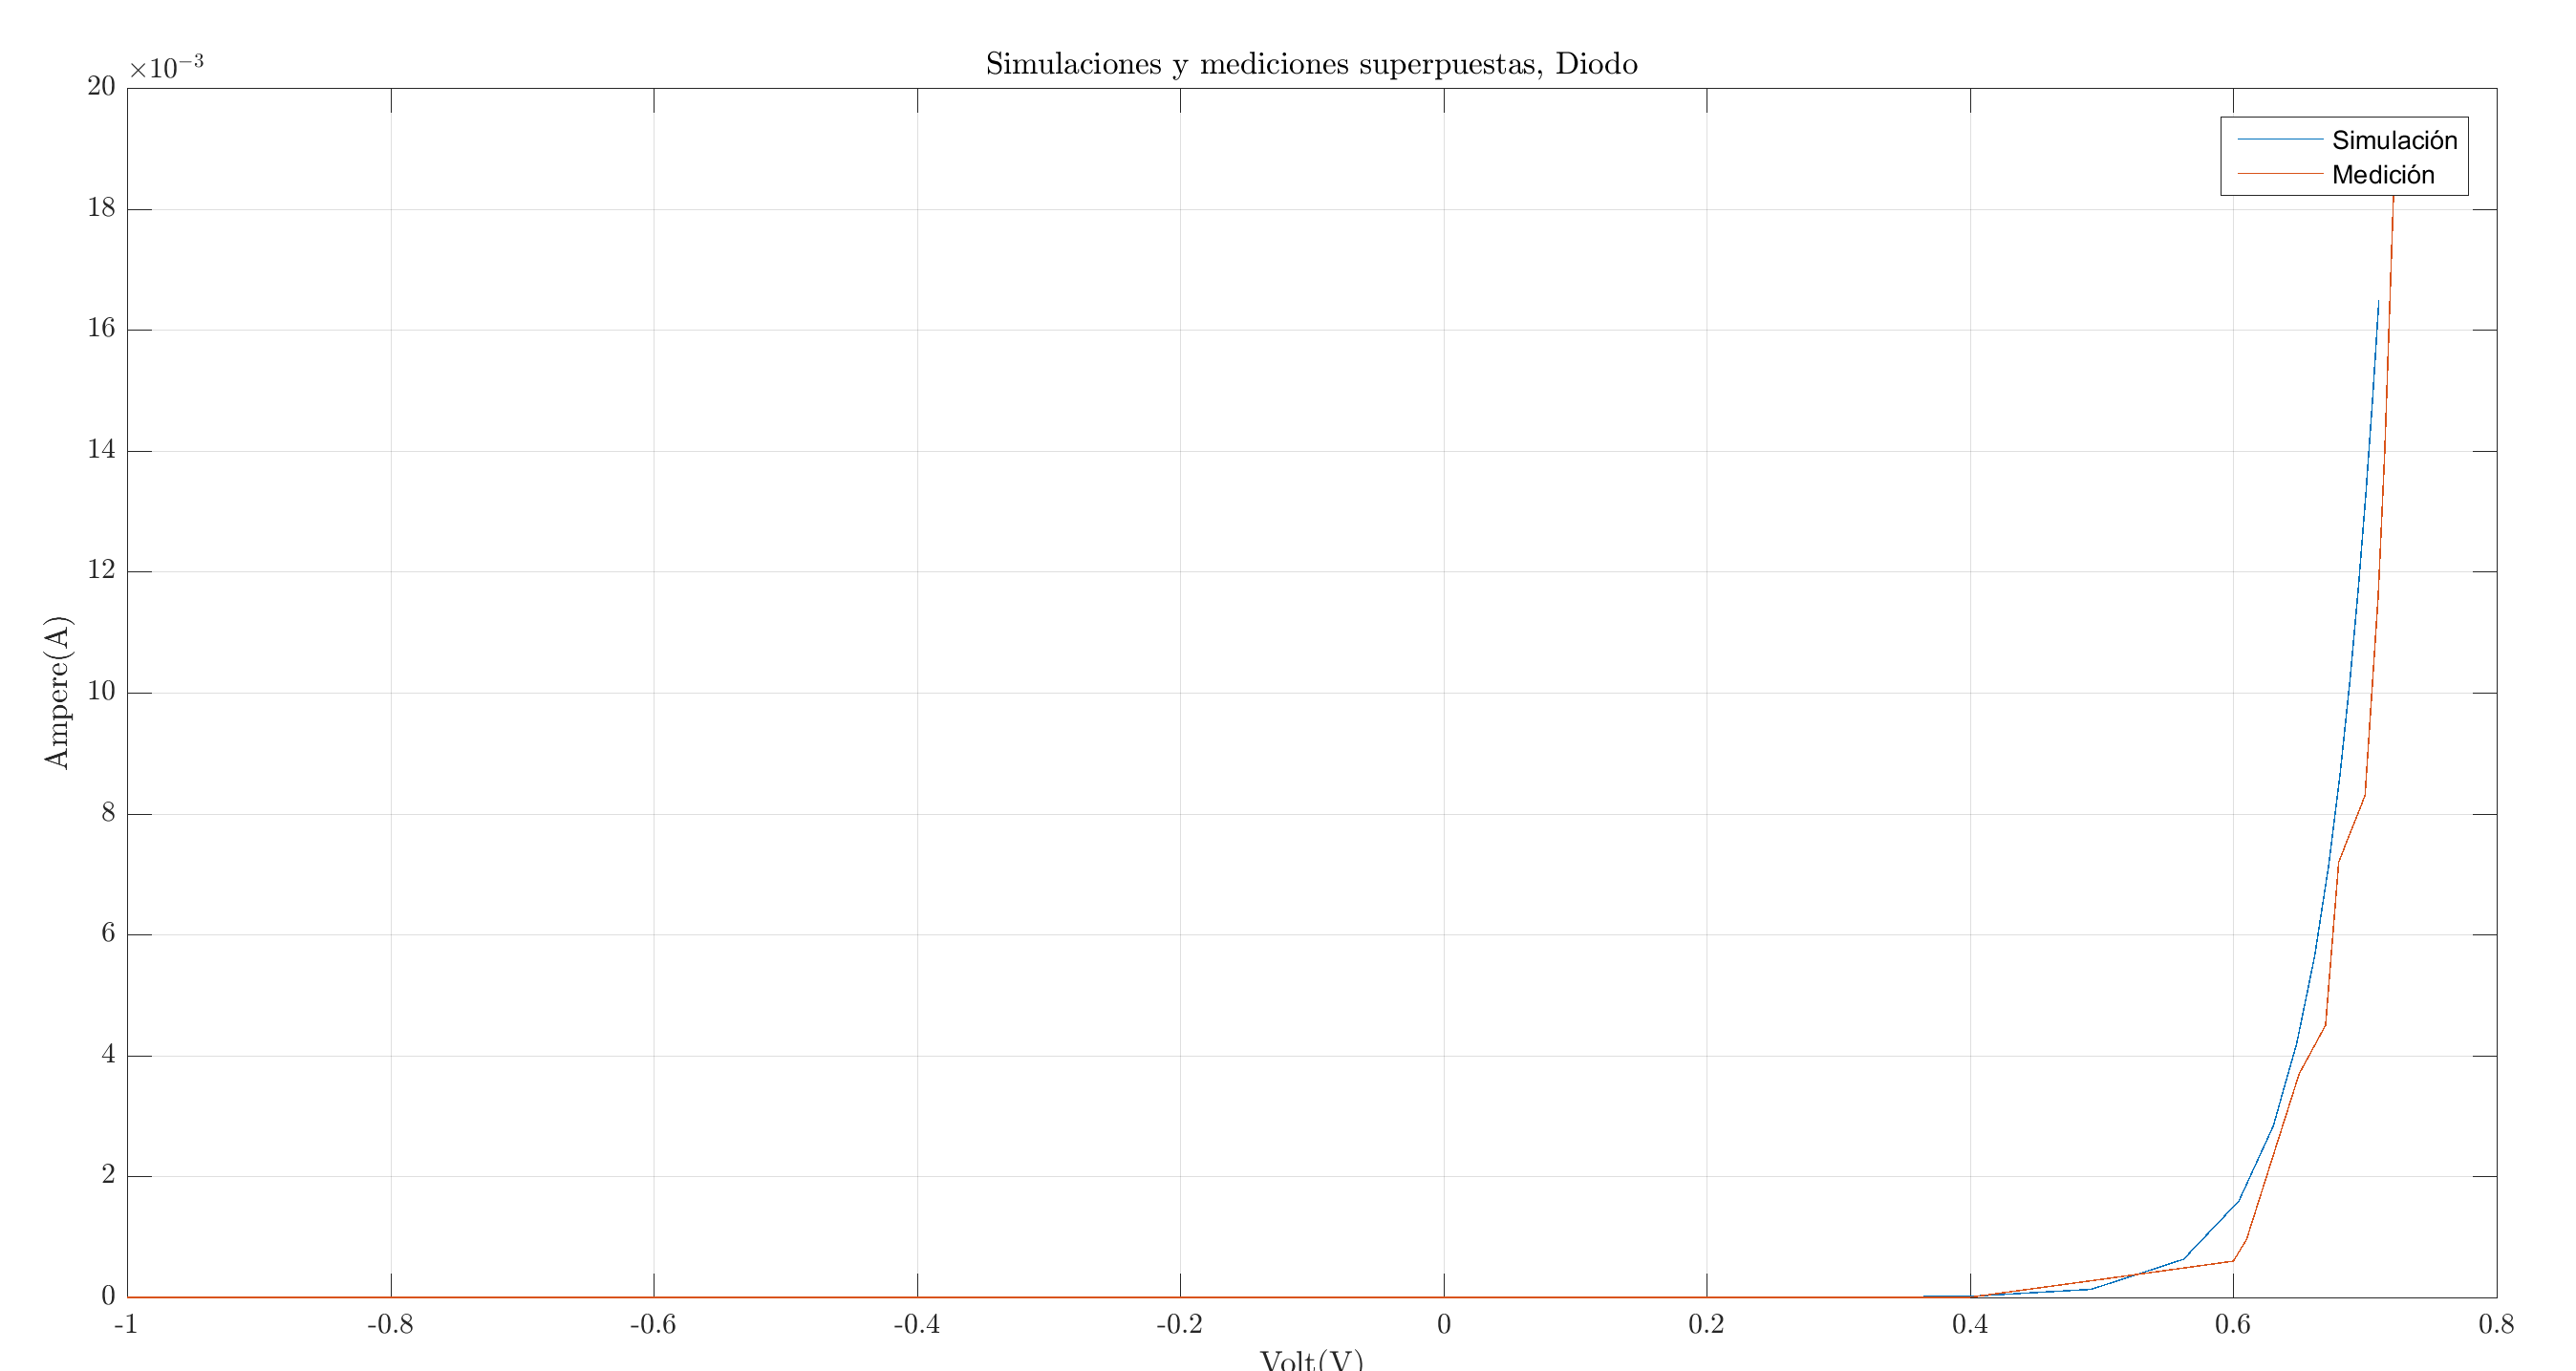
\includegraphics[scale=0.2]{imagenes/diodo_simulacion_medicion.png}
	\caption{Simulación de la curva del diodo y medición superpuestas.}
	\label{fig:ej5_diodo_simulacion_medicion}
\end{figure}

	La curva simulada coincide con la medida, por lo que se verifica que el diodo cumple con el modelo ideal.\par
	Debe hacerse notar que  la corriente en valores inferiores a los 0.4V no pudo ser medida, ya que el tester arrojaba una medición de 0V en su mínima escala. Esto se corresponde con el modelo teórico del diodo ya que la corriente en estos valores de tensión será del orden de los micro ampere, medición que no podrá ser realizada con los tester del pañol.\par

\section{Curva del diodo Zener}

	El diodo Zenner utilizado fue un diodo Zener de 3,9 V, modelo 1N4730A. Sin embargo, las simluaciones en LTSPICE se hicieron con el modelo GP3V9 ya que no se pudo obtener el modelo del 1N4730A para el SPICE, por lo que se espera una diferencia entre las curvas simulada y la medida.\par
	Se utilizó una fuente de tensión continua, a la cual se la fue variando y se midió la tensión en el diodo y la corriente que circulaba por la resistencia con tester.\par
	
	El circuito propuesto para realizar las mediciones es el siguiente:
	
	\begin{figure}[H]	%zener, circuito propuesto
		\centering
		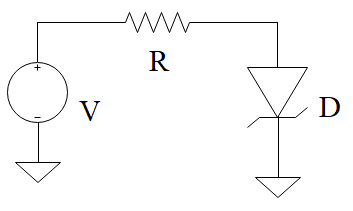
\includegraphics[scale=1.2]{imagenes/circuito_zener.png}
		\caption{Circuito propuesto para las mediciones del diodo Zener.}
		\label{fig:ej5_circuito_zener}
	\end{figure}

	Y las curvas resultantes de las mediciones y de las simulaciones fueron las siguientes:
	 
\begin{figure}[H]	%zener, curva
	\centering
	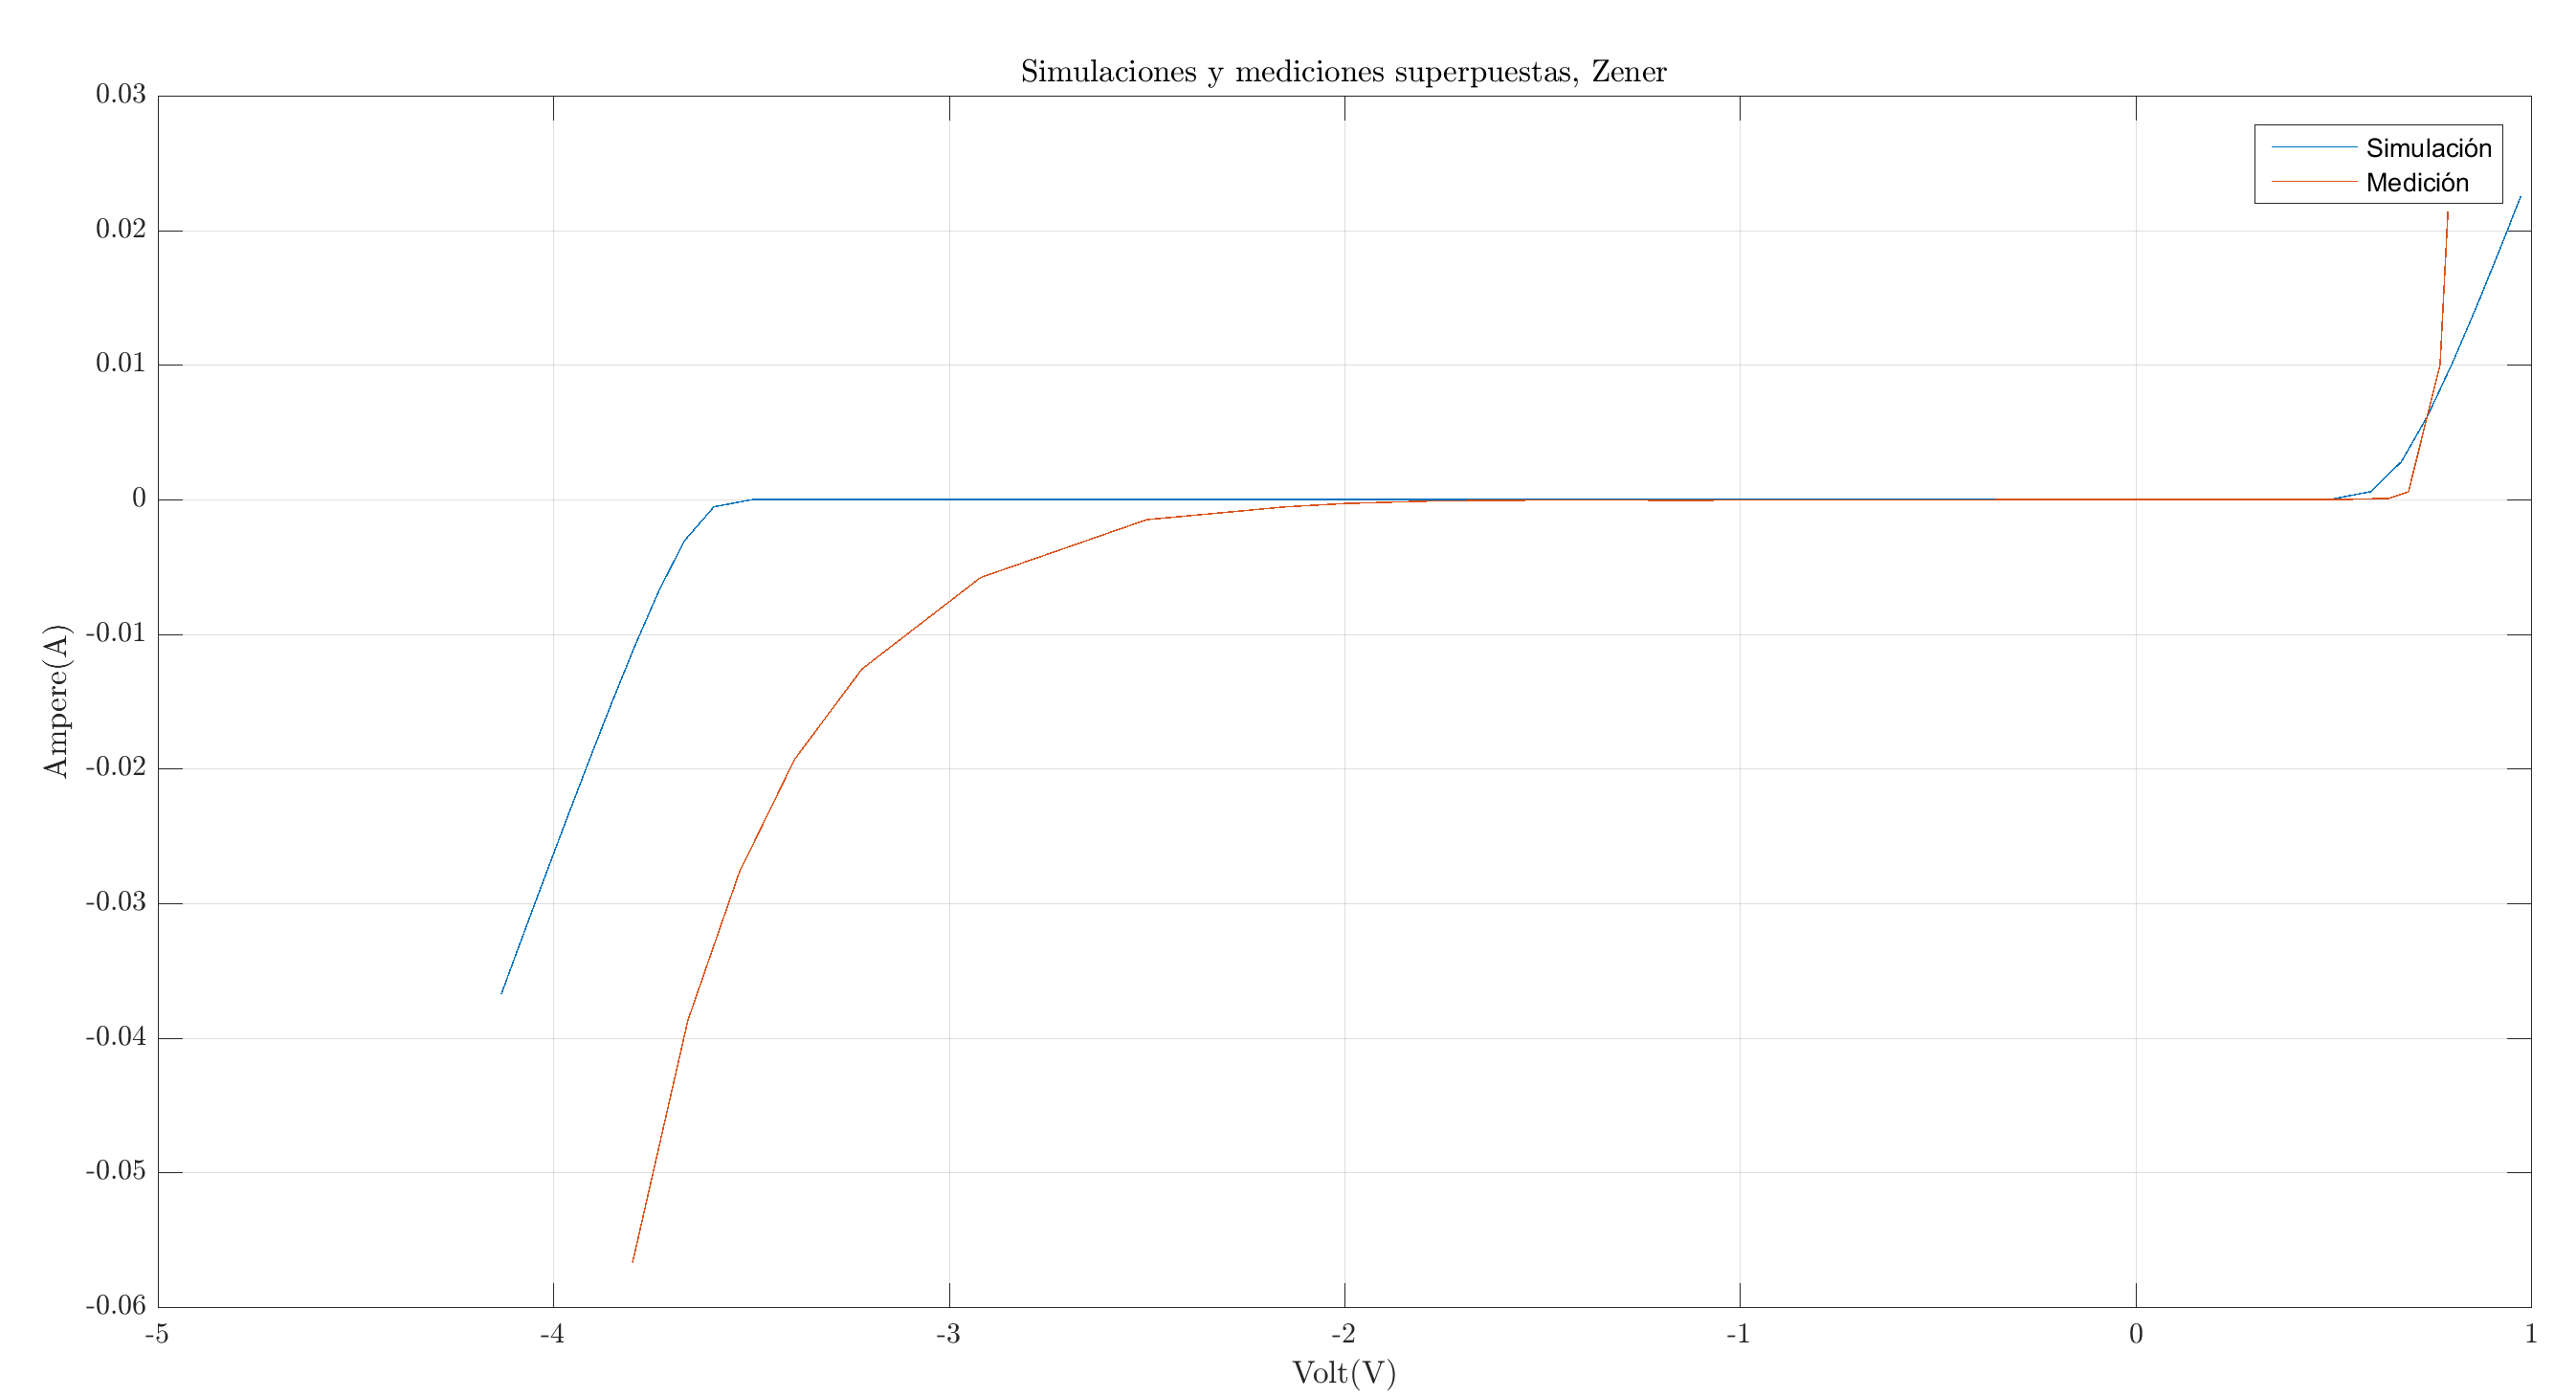
\includegraphics[scale=0.2]{imagenes/zener_simulacion_medicion.png}
	\caption{Simulación de la curva del zener y medición superpuestas.}
	\label{fig:ej5_zener_simulacion_medicion}
\end{figure}
	
	Como se puede notar, las curvas resultantes tienen la misma forma, la propia de un diodo zener, con una caída exponencial de la corriente cerca de la tensión de breakdown y una subida también exponencial para valores cercanos a 0.7. Sin embargo, debe hacerse notar que la tensión a partir de la cual comienza la caída abrupta para la simulación es exactamente 3.9 V, mientras que para el diodo medido, la caída comienza en valores cercanos a 3.5V.\par
	 Esto se cree que debe ser por la diferencia de modelos elegidos para la simulación y para la medición, siendo el diodo 1N4730A con el que se contaba un diodo de peor calidad en el sentido de que el ''codo'' característico del zener comienza para valores de tensiones relativamente bajos.\par 
Debe recordarse de la sección anterior que los valores de medición de corriente nulos no necesariamente lo son así, si no que estos son los valores que pudo arrojar un un tester común en mínima escala, pero que se estima que las corrientes circulantes serán del orden de los micro ampere. \par

\section{Curvas del transistor bipolar}

 El transistor utilizado fue un BC547. \par
 
 
 	El circuito propuesto para realizar las mediciones es el siguiente:
 	
	\begin{figure}[H]	%transistor, circuito propuesto
		\centering
		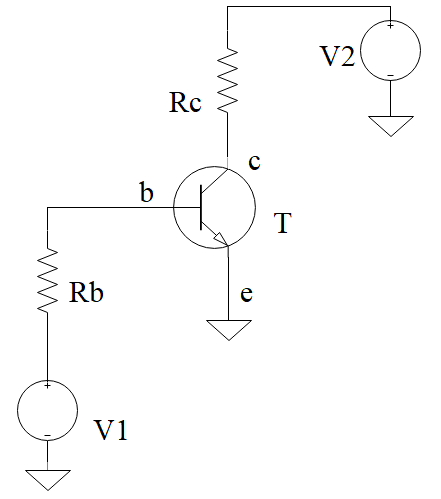
\includegraphics[scale=1.2]{imagenes/circuito_transistor.png}
		\caption{Circuito propuesto para las mediciones del transistor.}
		\label{fig:ej5_circuito_transistor}
	\end{figure}
	Para cada curva, se mantuvo la corriente de base constante. \par
	Las curvas resultantes de las mediciones y de las simulaciones fueron las siguientes:	
	
		%\begin{figure}[H]	%transistor, circuito propuesto
		%\centering
		%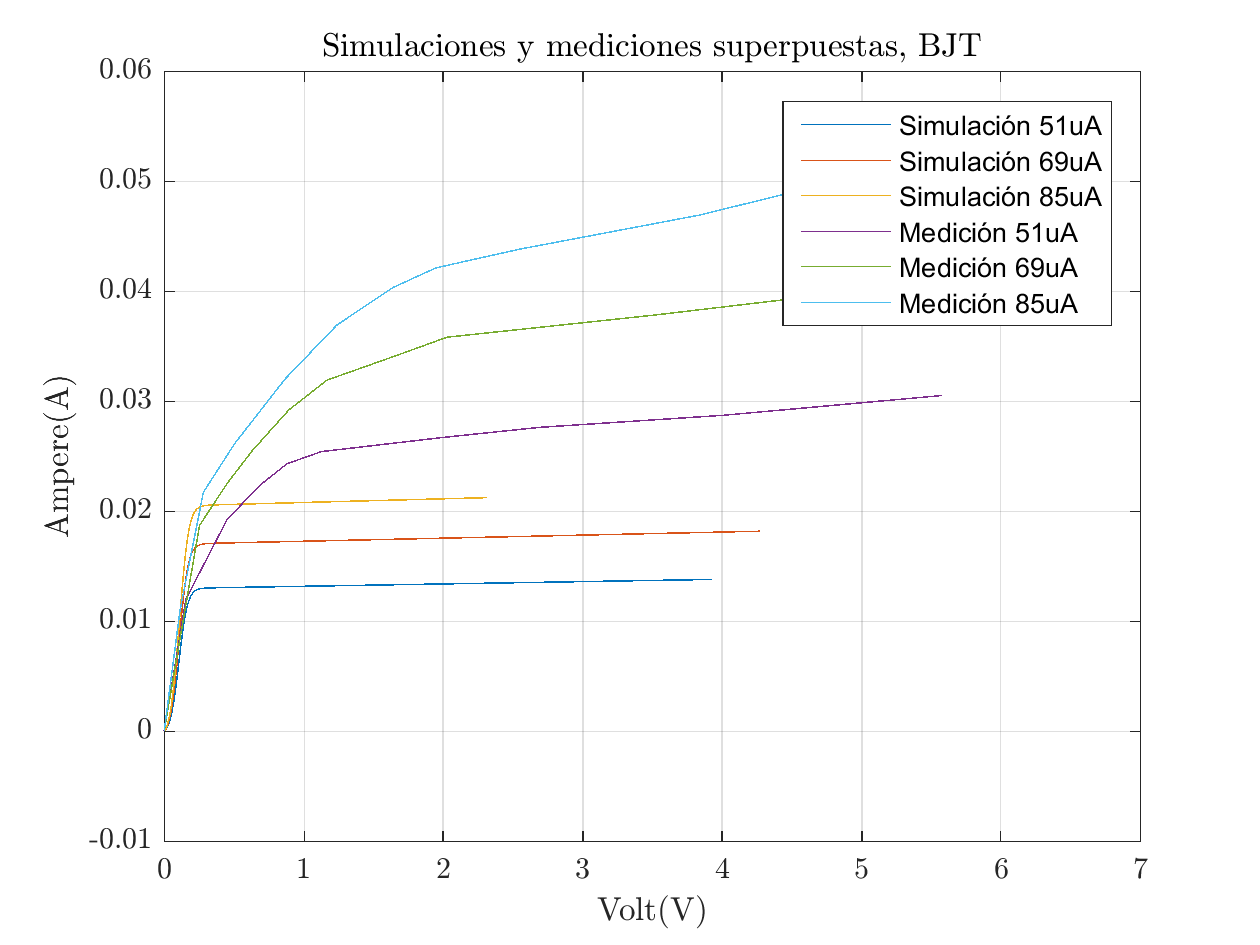
\includegraphics[scale=0.2]{imagenes/transistor_simulacion_medicion.png}
		%\caption{Simulación de la curva del transistor y medición superpuestas.}
		%\label{fig:ej5_transistor_simulacion_medicion}
	%\end{figure}
\end{document}
